% !TeX program = xelatex
\ifdefined\BookMaster\else
\documentclass[11pt,oneside]{article}
% !TeX program = xelatex
\usepackage[b5paper,left=22mm,right=22mm,top=20mm,bottom=22mm,footskip=11mm]{geometry}
\usepackage{fontspec}
\setmainfont{TeX Gyre Termes}
\setsansfont{TeX Gyre Heros}
\usepackage{amsmath,amssymb,mathtools,amsthm}
\renewcommand{\cdots}{\mathinner{\cdotp\cdotp\cdotp}}
\usepackage{graphicx,adjustbox,array,booktabs,longtable,multirow,enumitem,changepage,needspace}
\usepackage[table]{xcolor}
\usepackage{fancyhdr}
\raggedbottom
\interfootnotelinepenalty=10000
\newcommand{\BookFootnote}[2]{\begingroup\renewcommand{\thefootnote}{\fnsymbol{footnote}}\footnote[#1]{#2}\endgroup}
\newcommand{\BookFootnoteMark}[1]{\begingroup\renewcommand{\thefootnote}{\fnsymbol{footnote}}\footnotemark[#1]\endgroup}
\newcommand{\BookFootnoteText}[2]{\begingroup\renewcommand{\thefootnote}{\fnsymbol{footnote}}\footnotetext[#1]{#2}\endgroup}
\newenvironment{BookFloat}[1]{\par\addvspace{.6\baselineskip}\noindent\def\BookFloatID{#1}\begin{minipage}{\linewidth}\phantomsection\label{bookfloat:#1:start}}{\phantomsection\label{bookfloat:\BookFloatID:end}\end{minipage}\par\addvspace{.6\baselineskip}}

\usepackage[unicode,hidelinks]{hyperref}
\pagestyle{fancy}
\fancyhf{}
\newcommand{\BookFooter}{}
\fancyfoot[L]{\parbox[b]{\dimexpr\textwidth-15mm}{\footnotesize\BookFooter}}
\fancyfoot[R]{\footnotesize\thepage}
\renewcommand{\headrulewidth}{0pt}
\renewcommand{\footrulewidth}{0pt}
\setlength{\parindent}{0pt}
\setlength{\parskip}{0.2em}
\setlength{\emergencystretch}{3em}
\setlist{nosep,leftmargin=1.7em,labelsep=.65em}
\newif\ifBookNarrative
\BookNarrativetrue
\newenvironment{BookBody}{\setlength{\parindent}{0pt}}{}
\newcommand{\BookStatement}[1]{\par\addvspace{.6\baselineskip}\noindent #1\enspace\ignorespaces}
\newcommand{\BookLabel}[1]{\par\addvspace{.6\baselineskip}\needspace{3\baselineskip}\noindent\textbf{#1}\quad\ignorespaces}
\newcommand{\BookHeading}[1]{\par\addvspace{\baselineskip}\needspace{4\baselineskip}\noindent{\large\bfseries #1}\par\medskip}
\newcommand{\BookSubheading}[1]{\par\addvspace{.7\baselineskip}\needspace{3\baselineskip}\noindent{\bfseries #1}\par\smallskip}
\newcommand{\BookTextHeading}[1]{\par\addvspace{.7\baselineskip}\needspace{3\baselineskip}\noindent #1\par\smallskip}
\newcommand{\BookSectionTitle}[2]{\par\addvspace{1.2\baselineskip}\needspace{5\baselineskip}\noindent\colorbox{gray!25}{\sffamily\bfseries\small SECTION #1}\quad{\large\bfseries #2}\par\medskip}
\newcommand{\BookExerciseTitle}[1]{\par\addvspace{\baselineskip}\needspace{4\baselineskip}\noindent{\color{gray}\rule{1.5mm}{1.5mm}}\enspace{\large\bfseries Exercises #1}\par\medskip}
\newcommand{\BookBullet}[1]{\begin{list}{\textbullet}{\setlength{\leftmargin}{1.7em}\setlength{\labelwidth}{1em}\setlength{\labelsep}{.7em}\setlength{\topsep}{0pt}\setlength{\parsep}{0pt}\setlength{\itemsep}{0pt}}\item #1\end{list}}
\newcommand{\BookExercise}[2]{\begin{list}{\textbf{#1}}{\setlength{\leftmargin}{2.2em}\setlength{\labelwidth}{1.5em}\setlength{\labelsep}{.7em}\setlength{\topsep}{.15em}\setlength{\parsep}{0pt}\setlength{\itemsep}{0pt}}\item #2\end{list}}
\newcommand{\BookEnd}[1]{\unskip\nobreak\hfill\ensuremath{#1}}
\newcommand{\BookSource}[2]{\phantomsection\label{sourcepage:#1}} % Source-page anchors, retained through reflow.
\usepackage{multicol}
\usepackage{tikz}
\newcommand{\BookPartEntry}[2]{\par\noindent\makebox[17mm][l]{\bfseries Section #1}#2\par}
\newcommand{\BookPartTitle}[3]{\par\bigskip\noindent\begin{tikzpicture}\node[anchor=north west,inner sep=0pt,outer sep=0pt] (bookpart) at (0,0) {\begin{minipage}{\dimexpr\linewidth-.5pt}\hspace*{26mm}\begin{minipage}[t]{\dimexpr\linewidth-26mm}\begin{adjustbox}{max width=\linewidth}{\fontsize{20}{24}\selectfont\bfseries #2}\end{adjustbox}\par\vspace{6mm}\hrule\vspace{6mm}{\sffamily\footnotesize\setlength{\parskip}{.3em}#3}\vspace{3mm}\end{minipage}\end{minipage}};\path[shade,top color=gray!60,bottom color=white] (0,0) rectangle ([xshift=24mm]bookpart.south west);\node[anchor=north,font=\sffamily\bfseries\small] at (12mm,-2mm) {PART};\node[anchor=north,font=\sffamily\bfseries\Huge] at (12mm,-7mm) {#1};\end{tikzpicture}\par\bigskip}
\newsavebox{\BookMathBox}
\makeatletter
\newcommand{\BookInline}[1]{\leavevmode\hskip0pt\relax\begingroup\in@{\begin}{#1}\ifin@\sbox{\BookMathBox}{\(#1\)}\ifdim\wd\BookMathBox>\dimexpr\linewidth-1em\relax\resizebox{\dimexpr\linewidth-1em\relax}{!}{\usebox{\BookMathBox}}\else\(#1\)\fi\else\in@{\left}{#1}\ifin@\sbox{\BookMathBox}{\(#1\)}\ifdim\wd\BookMathBox>\dimexpr\linewidth-1em\relax\resizebox{\dimexpr\linewidth-1em\relax}{!}{\usebox{\BookMathBox}}\else\(#1\)\fi\else\(#1\)\fi\fi\endgroup\hskip0pt\relax}
\makeatother
\DeclareMathOperator{\Aut}{Aut}
\DeclareMathOperator{\End}{End}
\DeclareMathOperator{\Hom}{Hom}
\DeclareMathOperator{\GF}{GF}
\DeclareMathOperator{\irr}{irr}
\DeclareMathOperator{\lt}{lt}
\DeclareMathOperator{\lp}{lp}
\providecommand{\textcircled}[1]{\textnormal{(#1)}}

\begin{document}
\fi
\renewcommand{\BookFooter}{Section 39 Introduction to Extension Fields}
\pdfbookmark[0]{Section 39 Introduction to Extension Fields}{39_introduction_to_extension_fields}
\ifdefined\BookMaster\else\setcounter{page}{311}\fi
% Source PDF page 328; original printed page 311
\BookSource{328}{311}
\BookPartTitle{VIII}{Extension Fields}{\BookPartEntry{39}{Introduction to Extension Fields}
\BookPartEntry{40}{Algebraic Extensions}
\BookPartEntry{41}{Geometric Constructions\label{bookfootnote:328:2:ref}\BookFootnoteMark{2}}
\BookPartEntry{42}{Finite Fields}}
\BookFootnoteText{2}{\label{bookfootnote:328:2:text}Section 41 is not required for the remainder of the text.}

\BookNarrativetrue

\begin{BookBody}

\BookSectionTitle{39}{Introduction to Extension Fields}

\BookTextHeading{\textbf{Our Basic Goal Achieved}  }

\noindent We are now in a position to achieve our\textbf{ basic goal,} which, loosely stated, is to show that every nonconstant polynomial has a zero. This will be stated more precisely and proved in Theorem 39.3. We first introduce some new terminology for some old ideas.

\BookLabel{39.1 Definition} A field \BookInline{E} is an\textbf{ extension field of a field} \BookInline{F} if \BookInline{F\leq E.} \BookEnd{\blacksquare}

\begin{BookFloat}{39_introduction_to_extension_fields-p328-12}
\begin{center}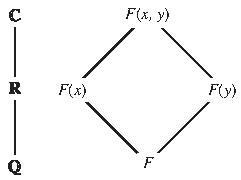
\includegraphics[width=0.331\linewidth,height=.8\textheight,keepaspectratio]{assets/p328_10.pdf}\end{center}
\begin{center}\small\textbf{39.2 Figure}\end{center}
\end{BookFloat}

Thus \BookInline{\mathbb{R}} is an extension field of \BookInline{\mathbb{Q},\allowbreak } and \BookInline{\mathbb{C}} is an extension field of both \BookInline{\mathbb{R}} and \BookInline{\mathbb{Q}.} As in the study of groups, it will often be convenient to use subfield diagrams to picture extension fields, the larger field being on top. We illustrate this in Fig. 39.2. (Recall that \BookInline{F(x)} is the field of quotients constructed from \BookInline{F[x].)} A configuration where there is just one single column of fields, as at the left-hand side of Fig. 39.2, is often referred to, without any precise definition, as a\textbf{ tower of fields.}

Now for our\textit{ basic goal!} This great and important result follows quickly and elegantly from the techniques we now have at our disposal.

\end{BookBody}

% Source PDF page 329; original printed page 312
\BookSource{329}{312}
\BookNarrativetrue

\begin{BookBody}

\BookLabel{39.3 Theorem} \textbf{(Kronecker’s Theorem) (Basic Goal)} Let \BookInline{F} be a field and let \BookInline{f(x)} be a nonconstant polynomial in \BookInline{F[x].} Then there exists an extension field \BookInline{E} of \BookInline{F} and an \BookInline{\alpha \in E} such that \BookInline{f(\alpha )= 0.}

\BookLabel{\textit{Proof}} By Theorem \BookInline{28.21,\allowbreak f(x)} has a factorization in \BookInline{F[x]} into polynomials that are irreducible over \BookInline{F.} Let \BookInline{p(x)} be an irreducible polynomial in such a factorization. It is clearly sufficient to find an extension field \BookInline{E} of \BookInline{F} containing an element \BookInline{\alpha } such that \BookInline{p(\alpha )= 0.}

By Theorem \BookInline{31.25,\allowbreak \langle p(x)\rangle } is a maximal ideal in \BookInline{F[x],\allowbreak } so \BookInline{F[x]/\langle p(x)\rangle } is a field. We claim that \BookInline{F} can be identified with a subfield of \BookInline{F[x]/\langle p(x)\rangle } in a natural way by use of the map \BookInline{\psi:F\to F[x]/\langle p(x)\rangle } given by

\begin{center}\begin{adjustbox}{max width=\linewidth}\BookInline{\displaystyle \psi (a)= a+ \langle p(x)\rangle}\end{adjustbox}\end{center}

\noindent for \BookInline{a\in F.} This map is one-to-one, for if \BookInline{\psi (a)= \psi (b),\allowbreak } that is, if \BookInline{a+ \langle p(x)\rangle = b+ \langle p(x)\rangle } for some \BookInline{a,\allowbreak b\in F,\allowbreak } then \BookInline{(a- b)\in \langle p(x)\rangle,\allowbreak } so \BookInline{a- b} must be a multiple of the polynomial \BookInline{p(x),\allowbreak } which is of degree \BookInline{\geq 1.} Now \BookInline{a,\allowbreak b\in F} implies that \BookInline{a- b} is in \BookInline{F.} Thus we must have \BookInline{a- b= 0,\allowbreak } so \BookInline{a= b.} We defined addition and multiplication in \BookInline{F[x]/\langle p(x)\rangle } by choosing any representatives, so we may choose \BookInline{a\in (a+ \langle p(x)\rangle ).} Thus \BookInline{\psi } is a homomorphism that maps \BookInline{F} one-to-one onto a subfield of \BookInline{F[x]/\langle p(x)\rangle.} We identify \BookInline{F} with \BookInline{\{a+ \langle p(x)\rangle \mid a\in F\}} by means of this map \BookInline{\psi.} Thus we shall view \BookInline{E= F[x]/\langle p(x)\rangle } as an extension field of \BookInline{F.} We have now manufactured our desired extension field \BookInline{E} of \BookInline{F.} It remains for us to show that \BookInline{E} contains a zero of \BookInline{p(x).}

\BookTextHeading{\textbf{HISTORICAL NOTE}  } \BookEnd{\blacksquare}

\noindent Leopold Kronecker is known for his insistence on constructibility of mathematical objects. As he noted, “God made the integers; all else is the work of man.” Thus, he wanted to be able to construct new “domains of rationality” (fields) by using only the existence of integers and indeterminates. He did not believe in starting with the real or complex numbers, because as far as he was concerned, those fields could not be determined in a constructive way. Hence in an 1881 paper, Kronecker created an extension field by simply adjoining to a given field a root \BookInline{\alpha } of an irreducible \BookInline{n}th degree polynomial \BookInline{p(x);} that is, his new field consisted of expressions rational in the original field elements and his new root \BookInline{\alpha } with the condition that \BookInline{p(\alpha )= 0.} The proof of the theorem presented in the text (Theorem 39.3) dates from the twentieth century.

Kronecker completed his dissertation in 1845 at the University of Berlin. For many years thereafter, he managed the family business, ultimately becoming financially independent. He then returned to Berlin, where he was elected to the Academy of Sciences and thus permitted to lecture at the university. On the retirement of Kummer, he became a professor at Berlin, and with Karl Weierstrass (1815–1897) directed the influential mathematics seminar.

Let us set

\begin{center}\begin{adjustbox}{max width=\linewidth}\BookInline{\displaystyle \alpha = x+ \langle p(x)\rangle ,\allowbreak }\end{adjustbox}\end{center}

\noindent so \BookInline{\alpha \in E.} Consider the evaluation homomorphism \BookInline{\phi _{\alpha }:F[x]\to E,\allowbreak } given by Theorem 27.4. If \BookInline{p(x)= a_{0}+ a_{1}x+ \cdots + a_{n}x^{n},\allowbreak } where \BookInline{a_{i}\in F,\allowbreak } then we have

\begin{center}\begin{adjustbox}{max width=\linewidth}\BookInline{\displaystyle \phi _{\alpha }(p(x))= a_{0}+ a_{1}(x+ \langle p(x)\rangle )+ \cdots + a_{n}(x+ \langle p(x)\rangle )^{n}}\end{adjustbox}\end{center}

\noindent in \BookInline{E= F[x]/\langle p(x)\rangle.} \textit{But we can compute in} \BookInline{F[x]/\langle p(x)\rangle } \textit{by choosing representatives, and} \BookInline{x} \textit{is} \BookInline{a} \textit{representative of the coset} \BookInline{\alpha = x+ \langle p(x)\rangle.} Therefore,

\begin{center}\begin{adjustbox}{max width=\linewidth}\BookInline{\displaystyle \begin{aligned}p(\alpha) &= \left( a_{0} + a_{1}x + \cdots + a_{n}x^{n} \right) + \langle p(x) \rangle \\&= p(x) + \langle p(x) \rangle = \langle p(x) \rangle = 0\end{aligned}}\end{adjustbox}\end{center}

\end{BookBody}

% Source PDF page 330; original printed page 313
\BookSource{330}{313}
\BookNarrativetrue

\begin{BookBody}

\noindent in \BookInline{F[x]/\langle p(x)\rangle.} We have found an element \BookInline{\alpha } in \BookInline{E= F[x]/\langle p(x)\rangle } such that \BookInline{p(\alpha )= 0,\allowbreak } and therefore \BookInline{f(\alpha )= 0.}\BookEnd{\blacklozenge}

We illustrate the construction involved in the proof of Theorem 39.3 by two examples.

\BookLabel{39.4 Example} Let \BookInline{F= \mathbb{R},\allowbreak } and let \BookInline{f(x)= x^{2}+ 1,\allowbreak } which is well known to have no zeros in \BookInline{\mathbb{R}} and thus is irreducible over \BookInline{\mathbb{R}} by Theorem 28.11. Then \BookInline{\langle x^{2}+ 1\rangle } is a maximal ideal in \BookInline{\mathbb{R}[x],\allowbreak } so \BookInline{\mathbb{R}[x]/\langle x^{2}+ 1\rangle } is a field. Identifying \BookInline{r\in \mathbb{R}} with \BookInline{r+ \langle x^{2}+ 1\rangle } in \BookInline{\mathbb{R}[x]/\langle x^{2}+ 1\rangle,\allowbreak } we can view \BookInline{\mathbb{R}} as a subfield of \BookInline{E= \mathbb{R}[x]/\langle x^{2}+ 1\rangle.} Let

\begin{center}\begin{adjustbox}{max width=\linewidth}\BookInline{\displaystyle \alpha = x+ \langle x^{2}+ 1\rangle .}\end{adjustbox}\end{center}

Computing in \BookInline{\mathbb{R}[x]/\langle x^{2}+ 1\rangle,\allowbreak } we find

\begin{center}\begin{adjustbox}{max width=\linewidth}\BookInline{\displaystyle \begin{aligned}\alpha ^{2}+ 1&= (x+ \langle x^{2}+ 1\rangle )^{2}+ (1+ \langle x^{2}+ 1\rangle ) \\ &= (x^{2}+ 1)+ \langle x^{2}+ 1\rangle = 0.\end{aligned}}\end{adjustbox}\end{center}

Thus \BookInline{\alpha } is a zero of \BookInline{x^{2}+ 1.} We shall identify \BookInline{\mathbb{R}[x]/\langle x^{2}+ 1\rangle } with \BookInline{\mathbb{C}} near the close of this section\BookInline{.}\BookEnd{\blacktriangle}

\BookLabel{39.5 Example} Let \BookInline{F= \mathbb{Q},\allowbreak } and consider \BookInline{f(x)= x^{4}- 5x^{2}+ 6.} This time \BookInline{f(x)} factors in \BookInline{\mathbb{Q}[x]} into \BookInline{(x^{2}- 2)(x^{2}- 3),\allowbreak } both factors being irreducible over \BookInline{\mathbb{Q},\allowbreak } as we have seen. We can start with \BookInline{x^{2}- 2} and construct an extension field \BookInline{E} of \BookInline{\mathbb{Q}} containing \BookInline{\alpha } such that \BookInline{\alpha ^{2}- 2= 0,\allowbreak } or we can construct an extension field \BookInline{K} of \BookInline{\mathbb{Q}} containing an element \BookInline{\beta } such that \BookInline{\beta ^{2}- 3= 0.} The construction in either case is just as in Example \BookInline{39.4.}\BookEnd{\blacktriangle}

\BookTextHeading{\textbf{Algebraic and Transcendental Elements}  }

\noindent As we said before, most of the rest of this text is devoted to the study of zeros of polynomials. We commence this study by putting an element of an extension field \BookInline{E} of a field \BookInline{F} into one of two categories.

\BookLabel{39.6 Definition} An element \BookInline{\alpha } of an extension field \BookInline{E} of a field \BookInline{F} is\textbf{ algebraic over} \BookInline{F} if \BookInline{f(\alpha )= 0} for some nonzero \BookInline{f(x)\in F[x].} If \BookInline{\alpha } is not algebraic over \BookInline{F,\allowbreak } then \BookInline{\alpha } is\textbf{ transcendental} \textbf{over} \BookInline{F.}\BookEnd{\blacksquare}

\BookLabel{39.7 Example} \BookInline{\mathbb{C}} is an extension field of \BookInline{\mathbb{Q}.} Since \BookInline{\sqrt{2}} is a zero of \BookInline{x^{2}- 2,\allowbreak } we see that \BookInline{\sqrt{2}} is an algebraic element over \BookInline{\mathbb{Q}.} Also\BookInline{,\allowbreak i} is an algebraic element over \BookInline{\mathbb{Q},\allowbreak } being a zero of \BookInline{x^{2}+ 1.}\BookEnd{\blacktriangle}

\BookLabel{39.8 Example} It is well known (but not easy to prove) that the real numbers \BookInline{\pi } and \BookInline{e} are transcendental over \BookInline{\mathbb{Q}.} Here \BookInline{e} is the base for the natural logarithms\BookInline{.}\BookEnd{\blacktriangle}

Just as we do not speak simply of an\textit{ irreducible polynomial,} but rather of an\textit{ ir}\textit{reducible polynomial over} \BookInline{F,\allowbreak } similarly we don’t speak simply of an\textit{ algebraic element,} but rather of an\textit{ element algebraic over} \BookInline{F.} The following illustration shows the reason for this.

\BookLabel{39.9 Example} The real number \BookInline{\pi } is transcendental over \BookInline{\mathbb{Q},\allowbreak } as we stated in Example 39.8. However, \BookInline{\pi } is algebraic over \BookInline{\mathbb{R},\allowbreak } for it is a zero of \BookInline{(x- \pi )\in \mathbb{R}[x].}\BookEnd{\blacktriangle}

\BookLabel{39.10 Example} It is easy to see that the real number \BookInline{\sqrt{1}+ \sqrt{3}} is algebraic over \BookInline{\mathbb{Q}.} For if \BookInline{\alpha = \sqrt{1}+ \sqrt{3},\allowbreak } then \BookInline{\alpha ^{2}= 1+ \sqrt{3},\allowbreak } so \BookInline{\alpha ^{2}- 1= \sqrt{3}} and \BookInline{(\alpha ^{2}- 1)^{2}= 3.} Therefore \BookInline{\alpha ^{4}- 2\alpha ^{2}- 2= 0,\allowbreak } so \BookInline{\alpha } is a zero of \BookInline{x^{4}- 2x^{2}- 2,\allowbreak } which is in \BookInline{\mathbb{Q}[x].}\BookEnd{\blacktriangle}

To connect these ideas with those of number theory, we give the following definition.

\end{BookBody}

% Source PDF page 331; original printed page 314
\BookSource{331}{314}
\BookNarrativetrue

\begin{BookBody}

\BookLabel{39.11 Definition} An element of \BookInline{\mathbb{C}} that is algebraic over \BookInline{\mathbb{Q}} is an\textbf{ algebraic number.} A\textbf{ transcendental} \textbf{number} is an element of \BookInline{\mathbb{C}} that is transcendental over \BookInline{\mathbb{Q}.}\BookEnd{\blacksquare}

There is an extensive and elegant theory of algebraic numbers. (See the Bibliography.)

The next theorem gives a useful characterization of algebraic and transcendental elements over \BookInline{F} in an extension field \BookInline{E} of \BookInline{F.} It also illustrates the importance of our evaluation homomorphisms \BookInline{\phi _{\alpha }.} \textit{Note that once more we are describing our concepts in} \textit{terms of mappings}.

\BookLabel{39.12 Theorem} Let \BookInline{E} be an extension field of a field \BookInline{F} and let \BookInline{\alpha \in E.} Let \BookInline{\phi _{\alpha }:F[x]\to E} be the evaluation homomorphism of \BookInline{F[x]} into \BookInline{E} such that \BookInline{\phi _{\alpha }(a)= a} for \BookInline{a\in F} and \BookInline{\phi _{\alpha }(x)= \alpha.} Then \BookInline{\alpha } is transcendental over \BookInline{F} if and only if \BookInline{\phi _{\alpha }} gives an isomorphism of \BookInline{F[x]} with a subdomain of \BookInline{E,\allowbreak } that is, if and only if \BookInline{\phi _{\alpha }} is a one-to-one map.

\BookLabel{\textit{Proof}} The element \BookInline{\alpha } is transcendental over \BookInline{F} if and only if \BookInline{f(\alpha )\neq 0} for all nonzero \BookInline{f(x)\in } \BookInline{F[x],\allowbreak } which is true (by definition) if and only if \BookInline{\phi _{\alpha }(f(x))\neq 0} for all nonzero \BookInline{f(x)\in F[x],\allowbreak } which is true if and only if the kernel of \BookInline{\phi _{\alpha }} is \BookInline{\{0\},\allowbreak } that is, if and only if \BookInline{\phi _{\alpha }} is a one-to-one map\BookInline{.}\BookEnd{\blacklozenge}

\BookTextHeading{\textbf{The Irreducible Polynomial for} \ensuremath{\alpha} \textbf{over} \textit{\textbf{F}}     }

Consider the extension field \BookInline{\mathbb{R}} of \BookInline{\mathbb{Q}.} We know that \BookInline{\sqrt{2}} is algebraic over \BookInline{\mathbb{Q},\allowbreak } being a zero of \BookInline{x^{2}- 2.} Of course\BookInline{,\allowbreak \sqrt{2}} is also a zero of \BookInline{x^{3}- 2x} and of \BookInline{x^{4}- 3x^{2}+ 2= (x^{2}- 2)} \BookInline{(x^{2}- 1).} Both these other polynomials having \BookInline{\sqrt{2}} as a zero were multiples of \BookInline{x^{2}- 2.} The next theorem shows that this is an illustration of a general situation. This theorem plays a central role in our later work.

\BookLabel{39.13 Theorem} Let \BookInline{E} be a field extension of \BookInline{F,\allowbreak } and let \BookInline{\alpha \in E} be algebraic over \BookInline{F.} Then \BookInline{\{f(x)\in } \BookInline{F[x]|f(\alpha )= 0\}= \langle p(x)\rangle } for some polynomial \BookInline{p(x)\in F[x].} Furthermore\BookInline{,\allowbreak p(x)} is irreducible over \BookInline{F.}

\BookLabel{\textit{Proof}} Let \BookInline{I= \{f(x)\in F[x]\mid f(\alpha )= 0\}.} Then \BookInline{I} is the kernel of the evaluation homomorphism \BookInline{\phi _{\alpha }:F[x]\to E,\allowbreak } which implies that \BookInline{I} is an ideal in \BookInline{F[x].} By Theorem \BookInline{31.24,\allowbreak I} is a principal ideal generated by a polynomial \BookInline{p(x)\in F[x].} Thus \BookInline{I= \langle p(x)\rangle.}

It remains to show that \BookInline{p(x)} is irreducible over \BookInline{F.} The degree of \BookInline{p(x)} is at least 1, which implies that \BookInline{p(x)} is neither 0 nor a unit in \BookInline{F[x].} Suppose that \BookInline{p(x)= r(x)s(x)} is a factorization of \BookInline{p(x)} over the field \BookInline{F.} Then applying the evaluation homomorphism, either \BookInline{r(\alpha )= 0} or \BookInline{s(\alpha )= 0,\allowbreak } since \BookInline{E} is a field. We relabel \BookInline{r} and \BookInline{s,\allowbreak } if necessary, so that \BookInline{r(\alpha )= 0.} Then \BookInline{r(x)\in I= \langle p(x)\rangle.} Thus

\begin{center}\begin{adjustbox}{max width=\linewidth}\BookInline{\displaystyle p(x)= r(x)s(x)= p(x)r_{1}(x)s(x)}\end{adjustbox}\end{center}

\noindent for some \BookInline{r_{1}(x)\in F[x].} Canceling \BookInline{p(x)} shows that \BookInline{s(x)} is a unit. Therefore\BookInline{,\allowbreak p(x)} is irreducible\BookInline{.}\BookEnd{\blacklozenge}

By multiplying by a suitable constant in \BookInline{F,\allowbreak } we can assume that the coefficient of the highest power of \BookInline{x} appearing in \BookInline{p(x)} of Theorem 39.13 is 1. Such a polynomial having 1 as the coefficient of the highest power of \BookInline{x} appearing is a\textbf{ monic polynomial.}

\BookLabel{39.14 Corollary} Let \BookInline{E} be an extension field of \BookInline{F,\allowbreak } and let \BookInline{\alpha \in E} be algebraic over \BookInline{F.} Then there is a unique irreducible polynomial \BookInline{p(x)\in F[x]} such that \BookInline{p(x)} is monic\BookInline{,\allowbreak p(\alpha )= 0,\allowbreak } and for any polynomial \BookInline{f(x)\in F[x]} with \BookInline{f(\alpha )= 0,\allowbreak p(x)} divides \BookInline{f(x).}

\BookLabel{\textit{Proof}} Let \BookInline{p(x)} be the polynomial of Theorem 39.13. By multiplying \BookInline{p(x)} with an appropriate element of \BookInline{F,\allowbreak } we can assume that \BookInline{p(x)} is monic. Since \BookInline{\{f(x)\mid f(\alpha )= 0\}= \langle p(x)\rangle,\allowbreak p(\alpha )= } 0 and for any \BookInline{f(x)\in F[x]} with \BookInline{f(\alpha )= 0,\allowbreak p(x)} divides \BookInline{f(x).}

\end{BookBody}

% Source PDF page 332; original printed page 315
\BookSource{332}{315}
\BookNarrativetrue

\begin{BookBody}

You are asked to prove uniqueness in Exercise 38. \BookEnd{\blacklozenge}

\BookLabel{39.15 Definition} Let \BookInline{E} be a field extension of a field \BookInline{F,\allowbreak } and let \BookInline{\alpha \in E} be algebraic over \BookInline{F.} The unique monic polynomial \BookInline{p(x)} in Corollary 39.14 is called the\textbf{ irreducible polynomial for} \BookInline{\alpha } \textbf{over} \BookInline{F} or the\textbf{ minimal polynomial for} \BookInline{\alpha } \textbf{over} \BookInline{F,\allowbreak } and it is denoted irr\BookInline{(\alpha,\allowbreak F).} The degree of the polynomial irr\BookInline{(\alpha,\allowbreak F)} is called the\textbf{ degree of} \BookInline{\alpha } \textbf{over} \BookInline{F} and this number is denoted by deg\BookInline{(\alpha,\allowbreak F).}\BookEnd{\blacksquare}

\BookLabel{39.16 Example} We know that irr\BookInline{(\sqrt{2},\allowbreak \mathbb{Q})= x^{2}- 2.} Referring to Example 39.10, we see that for \BookInline{\alpha = } \BookInline{\sqrt{1}+ \sqrt{3}} in \BookInline{\mathbb{R},\allowbreak \alpha } is a zero of \BookInline{x^{4}- 2x^{2}- 2,\allowbreak } which is in \BookInline{\mathbb{Q}[x].} Since \BookInline{x^{4}- 2x^{2}- 2} is irreducible over \BookInline{\mathbb{Q}(}by Eisenstein with \BookInline{p= 2,\allowbreak } or by application of the technique of Example 28.15), we see that

\begin{center}\begin{adjustbox}{max width=\linewidth}\BookInline{\displaystyle \;\text{irr}\;(\sqrt{1}+ \sqrt{3},\allowbreak \mathbb{Q})= x^{4}- 2x^{2}- 2.}\end{adjustbox}\end{center}

Thus \BookInline{\sqrt{1}+ \sqrt{3}} is algebraic of degree 4 over \BookInline{\mathbb{Q}.} \BookEnd{\blacktriangle}

Just as we must speak of an element \BookInline{\alpha } as\textit{ algebraic over} \BookInline{F} rather than simply as \textit{algebraic,} we must speak of the\textit{ degree of} \BookInline{\alpha } \textit{over} \BookInline{F} rather than the\textit{ degree of} \BookInline{\alpha.} To take a trivial illustration\BookInline{,\allowbreak \sqrt{2}\in \mathbb{R}} is algebraic of degree 2 over \BookInline{\mathbb{Q}} but algebraic of degree 1 over \BookInline{\mathbb{R},\allowbreak } for irr\BookInline{(\sqrt{2},\allowbreak \mathbb{R})= x- \sqrt{2}.}

The quick development of the theory here is due to the machinery of homomorphisms and ideal theory that we now have at our disposal. Note especially our constant use of the evaluation homomorphisms \BookInline{\phi _{\alpha }.}

\BookTextHeading{\textbf{Simple Extensions}  }

\noindent Let \BookInline{E} be an extension field of a field \BookInline{F,\allowbreak } and let \BookInline{\alpha \in E.} Let \BookInline{\phi _{\alpha }} be the evaluation homomorphism of \BookInline{F[x]} into \BookInline{E} with \BookInline{\phi _{\alpha }(a)= a} for \BookInline{a\in F} and \BookInline{\phi _{\alpha }(x)= \alpha,\allowbreak } as in Theorem 27.4. We use two cases to define the field \BookInline{F(\alpha ).}

\textbf{Case I} \textit{Suppose} \BookInline{\alpha } \textit{is algebraic over} \BookInline{F.} Then as in Corollary 39.14, the kernel of \BookInline{\phi _{\alpha }} is \BookInline{\langle }irr\BookInline{(\alpha,\allowbreak F)\rangle } and by Theorem \BookInline{31.25,\allowbreak \langle }irr\BookInline{(\alpha,\allowbreak F)\rangle } is a maximal ideal of \BookInline{F[x].} Therefore\BookInline{,\allowbreak F[x]/\langle }irr\BookInline{(\alpha,\allowbreak F)\rangle } is a field and is isomorphic to the image \BookInline{\phi _{\alpha }[F[x]]} in \BookInline{E.} This subfield \BookInline{\phi _{\alpha }[F[x]]} of \BookInline{E} is then the smallest subfield of \BookInline{E} containing \BookInline{F} and \BookInline{\alpha.} We shall denote this field by \BookInline{F(\alpha ).}

\textbf{Case II} \textit{Suppose} \BookInline{\alpha } \textit{is transcendental over} \BookInline{F.} Then by Theorem \BookInline{39.12,\allowbreak \phi _{\alpha }} gives an isomorphism of \BookInline{F[x]} with a subdomain of \BookInline{E.} Thus in this case \BookInline{\phi _{\alpha }[F[x]]} is\textit{ not} a field but an integral domain that we shall denote by \BookInline{F[\alpha ].} By Corollary \BookInline{26.9,\allowbreak E} contains a field of quotients of \BookInline{F[\alpha ],\allowbreak } which is thus the smallest subfield of \BookInline{E} containing \BookInline{F} and \BookInline{\alpha.} As in Case I, we denote this field by \BookInline{F(\alpha ).}

\BookLabel{39.17 Example} Since \BookInline{\pi } is transcendental over \BookInline{\mathbb{Q},\allowbreak } the field \BookInline{\mathbb{Q}(\pi )} is isomorphic to the field \BookInline{\mathbb{Q}(x)} of rational functions over \BookInline{\mathbb{Q}} in the indeterminate \BookInline{x.} Thus from a structural viewpoint, an element that is transcendental over a field \BookInline{F} behaves as though it were an indeterminate over \BookInline{F.}\BookEnd{\blacktriangle}

\BookLabel{39.18 Definition} An extension field \BookInline{E} of a field \BookInline{F} is a\textbf{ simple extension of} \BookInline{F} if \BookInline{E= F(\alpha )} for some \BookInline{\alpha \in E.}\BookEnd{\blacksquare}

Many important results appear throughout this section. We have now developed so much machinery that results are starting to pour out of our efficient plant at an alarming 
% Source PDF page 333; original printed page 316
\BookSource{333}{316}
rate. The next theorem gives us insight into the nature of the field \BookInline{F(\alpha )} in the case where \BookInline{\alpha } is algebraic over \BookInline{F.}

\end{BookBody}

\BookNarrativetrue

\begin{BookBody}

\BookLabel{39.19 Theorem} Let \BookInline{E= F(\alpha )} be a simple extension of a field \BookInline{F} with \BookInline{\alpha } algebraic over \BookInline{F.} Let \BookInline{n= } deg\BookInline{(\alpha,\allowbreak F).} Then every \BookInline{\beta \in F(\alpha )} can be uniquely expressed in the form

\begin{center}\begin{adjustbox}{max width=\linewidth}\BookInline{\displaystyle \beta = b_{0}+ b_{1}\alpha + b_{2}\alpha ^{2}+ \cdots + b_{n- 1}\alpha ^{n- 1},\allowbreak }\end{adjustbox}\end{center}

\noindent where the \BookInline{b_{i}} are in \BookInline{F.}

\BookLabel{\textit{Proof}} Let \BookInline{\beta \in F(\alpha ).} Then \BookInline{\beta = f(\alpha )} for some polynomial \BookInline{f(x)\in F[x]} by the definition of \BookInline{F[\alpha ].} The division algorithm says that there are unique polynomials \BookInline{q(x),\allowbreak r(x)\in F[x]} such that either \BookInline{r(x)= 0} or the degree of \BookInline{r(x)} is less than \BookInline{n,\allowbreak } and

\begin{center}\begin{adjustbox}{max width=\linewidth}\BookInline{\displaystyle f(x)= \;\text{irr}\;(\alpha ,\allowbreak F)q(x)+ r(x).}\end{adjustbox}\end{center}

\noindent Applying the evaluation homomorphism \BookInline{\phi _{\alpha },\allowbreak } we see that \BookInline{f(\alpha )= r(\alpha ).} Thus

\begin{center}\begin{adjustbox}{max width=\linewidth}\BookInline{\displaystyle \beta = f(\alpha )= r(\alpha )= b_{0}+ b_{1}\alpha + b_{2}\alpha ^{2}+ \cdots + b_{n- 1}\alpha ^{n- 1}}\end{adjustbox}\end{center}

\noindent for some elements \BookInline{b_{i}} in \BookInline{F.}

To show uniqueness, we assume that \BookInline{s(x)\in F[x]} is any polynomial with \BookInline{r(\alpha )= } \BookInline{s(\alpha ),\allowbreak } and \BookInline{s(x)} is either zero or else its degree is less than \BookInline{n.} Let \BookInline{d(x)= r(x)- s(x).} Then \BookInline{d(\alpha )= 0,\allowbreak } and either \BookInline{d(x)= 0} or deg\BookInline{(d(x))<n.} Since the degree of the minimal polynomial for \BookInline{\alpha } over \BookInline{F} is \BookInline{n,\allowbreak d(x)} is the zero polynomial and \BookInline{r(x)= s(x).} Thus the representation of \BookInline{\beta } as

\begin{center}\begin{adjustbox}{max width=\linewidth}\BookInline{\displaystyle \beta = b_{0}+ b_{1}\alpha + b_{2}\alpha ^{2}+ \cdots + b_{n- 1}\alpha ^{n- 1},\allowbreak }\end{adjustbox}\end{center}

\noindent where the \BookInline{b_{i}} are in \BookInline{F,\allowbreak } is unique. \BookEnd{\blacklozenge}

\noindent We give an impressive example illustrating Theorem 39.19.

\BookLabel{39.20 Example} The polynomial \BookInline{p(x)= x^{2}+ x+ 1} in \BookInline{\mathbb{Z}_{2}[x]} is irreducible over \BookInline{\mathbb{Z}_{2}} by Theorem 28.11, since neither element 0 nor element 1 of \BookInline{\mathbb{Z}_{2}} is a zero of \BookInline{p(x).} By Theorem 39.3, we know that there is an extension field \BookInline{E} of \BookInline{\mathbb{Z}_{2}} containing a zero \BookInline{\alpha } of \BookInline{x^{2}+ x+ 1.} By Theorem \BookInline{39.19,\allowbreak \mathbb{Z}_{2}(\alpha )} has as elements \BookInline{0+ 0\alpha,\allowbreak 1+ 0\alpha,\allowbreak 0+ 1\alpha,\allowbreak } and \BookInline{1+ 1\alpha,\allowbreak } that is, 0, \BookInline{1,\allowbreak \alpha,\allowbreak } and \BookInline{1+ \alpha.} \textit{This gives us} \BookInline{a} \textit{new finite} \BookInline{\text{fi}eld,\allowbreak } \textit{of four elements!} The addition and multiplication tables for this field are shown in Tables 39.21 and 39.22. For example, to compute \BookInline{(1+ \alpha )(1+ \alpha )} in \BookInline{\mathbb{Z}_{2}(\alpha ),\allowbreak } we observe that since \BookInline{p(\alpha )= \alpha ^{2}+ \alpha + 1= 0,\allowbreak } then

\begin{center}\begin{adjustbox}{max width=\linewidth}\BookInline{\displaystyle \alpha ^{2}= - \alpha - 1= \alpha + 1.}\end{adjustbox}\end{center}

\noindent Therefore,

\begin{center}\begin{adjustbox}{max width=\linewidth}\BookInline{\displaystyle (1+ \alpha )(1+ \alpha )= 1+ \alpha + \alpha + \alpha ^{2}= 1+ \alpha ^{2}= 1+ \alpha + 1= \alpha .}\end{adjustbox}\end{center} \BookEnd{\blacktriangle}

We can use Theorem 39.19 to fulfill our promise of Example 39.4 and show that \BookInline{\mathbb{R}[x]/\langle x^{2}+ 1\rangle } is isomorphic to the field \BookInline{\mathbb{C}} of complex numbers. We saw in Example 39.4 that we can view \BookInline{\mathbb{R}[x]/\langle x^{2}+ 1\rangle } as an extension field of \BookInline{\mathbb{R}.} Let

\begin{BookFloat}{39_introduction_to_extension_fields-p333-20}
\begin{center}
\begin{minipage}[t]{0.4776\linewidth}\vspace{0pt}\begin{center}\small\textbf{39.21 Table}\end{center}
\begin{center}\begin{adjustbox}{max width=\linewidth}
\renewcommand{\arraystretch}{1.2}\setlength{\tabcolsep}{5pt}
\begin{tabular}{c|c|c|c|c}
\BookInline{+ } & 0 & 1 & \BookInline{\alpha } & \BookInline{1+ \alpha }\\\hline
0 & 0 & 1 & \BookInline{\alpha } & \BookInline{1+ \alpha }\\\hline
1 & 1 & 0 & \BookInline{1+ \alpha } & \BookInline{\alpha }\\\hline
\BookInline{\alpha } & \BookInline{\alpha } & \BookInline{1+ \alpha } & 0 & 1\\\hline
\BookInline{1+ \alpha } & \BookInline{1+ \alpha } & \BookInline{\alpha } & 1 & 0\\
\end{tabular}
\end{adjustbox}\end{center}\end{minipage}\hfill\begin{minipage}[t]{0.4776\linewidth}\vspace{0pt}\begin{center}\small\textbf{39.22 Table}\end{center}
\begin{center}\begin{adjustbox}{max width=\linewidth}
\renewcommand{\arraystretch}{1.2}\setlength{\tabcolsep}{5pt}
\begin{tabular}{c|c|c|c|c}
 & 0 & 1 & \BookInline{\alpha } & \BookInline{1+ \alpha }\\\hline
0 & 0 & 0 & 0 & 0\\\hline
1 & 0 & 1 & \BookInline{\alpha } & \BookInline{1+ \alpha }\\\hline
\BookInline{\alpha } & 0 & \BookInline{\alpha } & \BookInline{1+ \alpha } & 1\\\hline
\BookInline{1+ \alpha } & 0 & \BookInline{1+ \alpha } & 1 & \BookInline{\alpha }\\
\end{tabular}
\end{adjustbox}\end{center}\end{minipage}
\end{center}
\end{BookFloat}

\end{BookBody}

% Source PDF page 334; original printed page 317
\BookSource{334}{317}
\BookNarrativetrue

\begin{BookBody}

\begin{center}\begin{adjustbox}{max width=\linewidth}\BookInline{\displaystyle \alpha = x+ \langle x^{2}+ 1\rangle .}\end{adjustbox}\end{center}

\noindent Then \BookInline{\mathbb{R}(\alpha )= \mathbb{R}[x]/\langle x^{2}+ 1\rangle } and consists of all elements of the form \BookInline{a+ b\alpha } for \BookInline{a,\allowbreak b\in } \BookInline{\mathbb{R},\allowbreak } by Theorem 39.19. But since \BookInline{\alpha ^{2}+ 1= 0,\allowbreak } we see that \BookInline{\alpha } plays the role of \BookInline{i\in \mathbb{C},\allowbreak } and \BookInline{a+ b\alpha } plays the role of \BookInline{(a+ } \textit{bi}\BookInline{)\; \in \mathbb{C}.} Thus \BookInline{\mathbb{R}(\alpha )\simeq \mathbb{C}.} \textit{This is the elegant algebraic} \textit{way to construct} \BookInline{\mathbb{C}} \textit{from} \BookInline{\mathbb{R}.}

\BookLabel{39.23 Corollary} Let \BookInline{E} be an extension field of \BookInline{F} and let \BookInline{\alpha \in E} be algebraic over \BookInline{F.} If deg\BookInline{(\alpha,\allowbreak F)= n,\allowbreak } then \BookInline{F(\alpha )} is a vector space over \BookInline{F} with dimension \BookInline{n} and basis \BookInline{\{1,\allowbreak \alpha,\allowbreak \alpha ^{2},\allowbreak...,\allowbreak \alpha ^{n- 1}\}.} Furthermore, every element \BookInline{\beta } of \BookInline{F(\alpha )} is algebraic over \BookInline{F} and deg\BookInline{(\beta,\allowbreak F)\leq } deg\BookInline{(\alpha,\allowbreak F).}

\BookLabel{\textit{Proof}} Since \BookInline{F} is a subfield of \BookInline{F(\alpha ),\allowbreak F(\alpha )} is a vector space over \BookInline{F.} Theorem 39.19 shows that the set \BookInline{\{1,\allowbreak \alpha,\allowbreak \alpha ^{2},\allowbreak...,\allowbreak \alpha ^{n- 1}\}} spans \BookInline{F(\alpha ).} If

\begin{center}\begin{adjustbox}{max width=\linewidth}\BookInline{\displaystyle 0= b_{0}(1)+ b_{1}\alpha + b_{2}\alpha ^{2}+ \cdots + b_{n- 1}\alpha ^{n- 1},\allowbreak }\end{adjustbox}\end{center}

\noindent by uniqueness of the coefficients in Theorem 39.19, each \BookInline{b_{i}} is 0. We have that \BookInline{\{1,\allowbreak \alpha,\allowbreak \alpha ^{2},\allowbreak...,\allowbreak \alpha ^{n- 1}\}} is linearly independent over \BookInline{F,\allowbreak } and therefore a basis of \BookInline{F(\alpha )} over \BookInline{F.} Thus the dimension of \BookInline{F(\alpha )} over \BookInline{F} is \BookInline{n= } deg\BookInline{(\alpha,\allowbreak F).}

For any \BookInline{\beta \in F(\alpha ),\allowbreak F\leq F(\beta )\leq F(\alpha ),\allowbreak } so any set of more than \BookInline{n} vectors in \BookInline{F(\beta )} is not linearly independent over \BookInline{F.} The set \BookInline{\{1,\allowbreak \beta,\allowbreak \beta ^{2},\allowbreak...,\allowbreak \beta ^{n}\}} either has fewer than \BookInline{n+ 1} elements or else it is not linearly independent over \BookInline{F.} In the first case\BookInline{,\allowbreak \beta ^{r}= \beta ^{s}} for some \BookInline{r\neq s} and in the second case, there are elements \BookInline{b_{i}\in F,\allowbreak } not all zero, such that

\begin{center}\begin{adjustbox}{max width=\linewidth}\BookInline{\displaystyle b_{0}(1)+ b_{1}\beta + b_{2}\beta ^{2}+ \cdots + b_{n}\beta ^{n}= 0.}\end{adjustbox}\end{center}

\noindent In either case, we see that \BookInline{\beta } is algebraic over \BookInline{F.} Furthermore the dimension of \BookInline{F(\beta )} over \BookInline{F,\allowbreak k,\allowbreak } is at most \BookInline{n} and we have

\begin{center}\begin{adjustbox}{max width=\linewidth}\BookInline{\displaystyle \;\text{deg}\;(\beta ,\allowbreak F)= k\leq n= \;\text{deg}\;(\alpha ,\allowbreak F).}\end{adjustbox}\end{center} \BookEnd{\blacklozenge}

\BookLabel{39.24 Example} The number \BookInline{i\in \mathbb{C}} has minimal polynomial \BookInline{x^{2}+ 1} over \BookInline{\mathbb{R}} and \BookInline{\mathbb{C}= \mathbb{R}(i).} By Corollary 39.23, for every complex number \BookInline{\beta,\allowbreak } deg\BookInline{(\beta,\allowbreak \mathbb{R})\leq 2.} This implies that every complex number that is not a real number is a zero of some irreducible polynomial of degree two in \BookInline{\mathbb{R}[x].} Of course, this fact can also be verified using the techniques of Example \BookInline{39.10.}\BookEnd{\blacktriangle}

\end{BookBody}

\BookNarrativefalse

\begin{BookBody}

\BookExerciseTitle{39}

\BookTextHeading{\textbf{Computations}}

\noindent In Exercises 1 through 5, show that the given number \BookInline{\alpha \in \mathbb{C}} is algebraic over \BookInline{\mathbb{Q}} by finding \BookInline{f(x)\in \mathbb{Q}[x]} such that \BookInline{f(\alpha )= 0.}

\BookExercise{3.}{\BookInline{1+ i}}

\BookExercise{1.}{\BookInline{1+ \sqrt{2}}}

\BookExercise{2.}{\BookInline{\sqrt{2}+ \sqrt{3}}}

\BookExercise{4.}{\BookInline{\sqrt{1 + \sqrt[3]{2}}}}

\BookExercise{5.}{\BookInline{\sqrt { \sqrt [ 3 ] { 2 } - i }}}

\noindent In Exercises 6 through 8, find irr\BookInline{(\alpha,\allowbreak \mathbb{Q})} and deg\BookInline{(\alpha,\allowbreak \mathbb{Q})} for the given algebraic number \BookInline{\alpha \in \mathbb{C}.} Be prepared to prove that your polynomials are irreducible over \BookInline{\mathbb{Q}} if challenged to do so.

\BookInline{\sqrt { ( \frac { 1 } { 3 } ) + \sqrt { 7 } }}

\begin{center}\begin{adjustbox}{max width=\linewidth}\BookInline{\displaystyle 6.\ \sqrt{3 - \sqrt{6}}}\end{adjustbox}\end{center}

\begin{center}\begin{adjustbox}{max width=\linewidth}\BookInline{\displaystyle 8.\sqrt{2}+ i}\end{adjustbox}\end{center}

\BookExercise{7.}{\BookInline{\sqrt { ( \frac { 1 } { 3 } ) + \sqrt { 7 } }}}

\end{BookBody}

% Source PDF page 335; original printed page 318
\BookSource{335}{318}
\BookNarrativefalse

\begin{BookBody}

\noindent In Exercises 9 through 16, classify the given \BookInline{\alpha \in \mathbb{C}} as algebraic or transcendental over the given field \BookInline{F.} If \BookInline{\alpha } is algebraic over \BookInline{F,\allowbreak } find deg\BookInline{(\alpha,\allowbreak F).}

\BookExercise{9.}{\BookInline{\alpha = i,\allowbreak F= \mathbb{Q}}}

\BookExercise{10.}{\BookInline{\alpha = 1+ i,\allowbreak F= \mathbb{R}}}

\BookExercise{11.}{\BookInline{\alpha = \sqrt{\pi },\allowbreak F= \mathbb{Q}}}

\BookExercise{12.}{\BookInline{\alpha = \sqrt{\pi },\allowbreak F= \mathbb{R}}}

\BookExercise{13.}{\BookInline{\alpha = \sqrt{\pi },\allowbreak F= \mathbb{Q}(\pi )}}

\BookExercise{14.}{\BookInline{\alpha = \pi ^{2},\allowbreak F= \mathbb{Q}}}

\BookExercise{15.}{\BookInline{\alpha = \pi ^{2},\allowbreak F= \mathbb{Q}(\pi )}}

\BookExercise{16.}{\BookInline{\alpha = \pi ^{2},\allowbreak F= \mathbb{Q}(\pi ^{3})}}

\BookExercise{17.}{Refer to Example 39.20 of the text. The polynomial \BookInline{x^{2}+ x+ 1} has a zero \BookInline{\alpha } in \BookInline{\mathbb{Z}_{2}(\alpha )} and thus must factor into a product of linear factors in \BookInline{(\mathbb{Z}_{2}(\alpha ))[x].} Find this factorization. [\textit{Hint:} Divide \BookInline{x^{2}+ x+ 1} by \BookInline{x- \alpha } by long division, using the fact that \BookInline{\alpha ^{2}= \alpha + 1.]}}

\BookExercise{18.}{\textbf{. a} Show that the polynomial \BookInline{x^{2}+ 1} is irreducible in \BookInline{\mathbb{Z}_{3}[x].}}

\BookExercise{b.}{Let \BookInline{\alpha } be a zero of \BookInline{x^{2}+ 1} in an extension field of \BookInline{\mathbb{Z}_{3}.} As in Example 39.20, give the multiplication and addition tables for the nine elements of \BookInline{\mathbb{Z}_{3}(\alpha ),\allowbreak } written in the order \BookInline{0,\allowbreak 1,\allowbreak 2,\allowbreak \alpha,\allowbreak 2\alpha,\allowbreak 1+ \alpha,\allowbreak 1+ 2\alpha,\allowbreak 2+ \alpha,\allowbreak } and \BookInline{2+ 2\alpha.}}

\BookTextHeading{\textbf{Concepts}}

\noindent In Exercises 19 through 22, correct the definition of the italicized term without reference to the text, if correction is needed, so that it is in a form acceptable for publication.

\BookExercise{19.}{An element \BookInline{\alpha } of an extension field \BookInline{E} of a field \BookInline{F} is\textit{ algebraic over} \BookInline{F} if and only if \BookInline{\alpha } is a zero of some polynomial.}

\BookExercise{20.}{An element \BookInline{\beta } of an extension field \BookInline{E} of a field \BookInline{F} is\textit{ transcendental over} \BookInline{F} if and only if \BookInline{\beta } is not a zero of any polynomial in \BookInline{F[x].}}

\BookExercise{21.}{A\textit{ monic polynomial in} \BookInline{F[x]} is one having all coefficients equal to 1.}

\BookExercise{22.}{A field \BookInline{E} is a\textit{ simple extension} of a subfield \BookInline{F} if and only if there exists some \BookInline{\alpha \in E} such that no proper subfield of \BookInline{E} contains \BookInline{\alpha.}}

\BookExercise{23.}{Determine whether each of the following is true or false.}

\BookExercise{a.}{The number \BookInline{\pi } is transcendental over \BookInline{\mathbb{Q}.}}

\BookExercise{b.}{\textbf{b}\BookInline{.\mathbb{C}} is a simple extension of \BookInline{\mathbb{R}.}}

\BookExercise{c.}{Every element of a field \BookInline{F} is algebraic over \BookInline{F.}}

\BookExercise{d.}{\textbf{d}\BookInline{.\mathbb{R}} is an extension field of \BookInline{\mathbb{Q}.}}

\BookExercise{e.}{\textbf{e}\BookInline{.\mathbb{Q}} is an extension field of \BookInline{\mathbb{Z}_{2}.}}

\BookExercise{f.}{Let \BookInline{\alpha \in \mathbb{C}} be algebraic over \BookInline{\mathbb{Q}} of degree \BookInline{n.} If \BookInline{f(\alpha )= 0} for nonzero \BookInline{f(x)\in \mathbb{Q}[x],\allowbreak } then deg \BookInline{(f(x))\geq n.}}

\BookExercise{g.}{Let \BookInline{\alpha \in \mathbb{C}} be algebraic over \BookInline{\mathbb{Q}} of degree \BookInline{n.} If \BookInline{f(\alpha )= 0} for nonzero \BookInline{f(x)\in \mathbb{R}[x],\allowbreak } then deg \BookInline{(f(x))\geq n.}}

\BookExercise{h.}{Every nonconstant polynomial in \BookInline{F[x]} has a zero in some extension field of \BookInline{F.}}

\BookExercise{i.}{Every nonconstant polynomial in \BookInline{F[x]} has a zero in every extension field of \BookInline{F.}}

\BookExercise{j.}{If \BookInline{x} is an indeterminate\BookInline{,\allowbreak \mathbb{Q}[\pi ]\simeq \mathbb{Q}[x].}}

\BookExercise{24.}{We have stated without proof that \BookInline{\pi } and \BookInline{e} are transcendental over \BookInline{\mathbb{Q}.}}

\BookExercise{a.}{Find a subfield \BookInline{F} of \BookInline{\mathbb{R}} such that \BookInline{\pi } is algebraic of degree 3 over \BookInline{F.}}

\BookExercise{b.}{Find a subfield \BookInline{E} of \BookInline{\mathbb{R}} such that \BookInline{e^{2}} is algebraic of degree 5 over \BookInline{E.}}

\BookExercise{25.}{\textbf{. a} Show that \BookInline{x^{3}+ x^{2}+ 1} is irreducible over \BookInline{\mathbb{Z}_{2}.}}

\BookExercise{b.}{Let \BookInline{\alpha } be a zero of \BookInline{x^{3}+ x^{2}+ 1} in an extension field of \BookInline{\mathbb{Z}_{2}.} Show that \BookInline{x^{3}+ x^{2}+ 1} factors into three linear factors in \BookInline{(\mathbb{Z}_{2}(\alpha ))[x]} by actually finding this factorization. [\textit{Hint:} Every element of \BookInline{\mathbb{Z}_{2}(\alpha )} is of the form}

\begin{center}\begin{adjustbox}{max width=\linewidth}\BookInline{\displaystyle a_{0}+ a_{1}\alpha + a_{2}\alpha ^{2}\;\text{for}\;a_{i}= 0,\allowbreak 1.}\end{adjustbox}\end{center}

Divide \BookInline{x^{3}+ x^{2}+ 1} by \BookInline{x- \alpha } by long division. Show that the quotient also has a zero in \BookInline{\mathbb{Z}_{2}(\alpha )} by simply trying the eight possible elements. Then complete the factorization.]

\end{BookBody}

% Continuation on source PDF page 336, preceding Section 40
\BookNarrativefalse

\begin{BookBody}

\BookExercise{26.}{Let \BookInline{E} be an extension field of \BookInline{\mathbb{Z}_{2}} and let \BookInline{\alpha \in E} be algebraic of degree 3 over \BookInline{\mathbb{Z}_{2}.} Classify the groups \BookInline{\langle \mathbb{Z}_{2}(\alpha ),\allowbreak + \rangle } and \BookInline{\langle (\mathbb{Z}_{2}(\alpha ))^{\ast },\allowbreak \cdot \rangle } according to the Fundamental Theorem of finitely generated abelian groups. As usual\BookInline{,\allowbreak (\mathbb{Z}_{2}(\alpha ))^{\ast }} is the set of nonzero elements of \BookInline{\mathbb{Z}_{2}(\alpha ).}}

\BookExercise{27.}{Definition 39.15 defined the terms\textbf{ irreducible polynomial for} \BookInline{\alpha } \textbf{over} \BookInline{F} and\textbf{ minimal polynomial for} \BookInline{\alpha } \textbf{over} \BookInline{F} to mean the same polynomial. Why are both designations appropriate?}

\BookLabel{\textit{Proof}} \textbf{ Synopsis}

\BookExercise{28.}{Give a two- or three-sentence synopsis of Theorem 39.3.}

\BookTextHeading{\textbf{Theory}}

\BookExercise{29.}{Let \BookInline{E} be an extension field of \BookInline{F,\allowbreak } and let \BookInline{\alpha,\allowbreak \beta \in E.} Suppose \BookInline{\alpha } is transcendental over \BookInline{F} but algebraic over \BookInline{F(\beta ).} Show that \BookInline{\beta } is algebraic over \BookInline{F(\alpha ).}}

\BookExercise{30.}{Let \BookInline{E} be an extension field of a finite field \BookInline{F,\allowbreak } where \BookInline{F} has \BookInline{q} elements. Let \BookInline{\alpha \in E} be algebraic over \BookInline{F} of degree \BookInline{n.} Prove that \BookInline{F(\alpha )} has \BookInline{q^{n}} elements.}

\BookExercise{31.}{\textbf{. a} Show that there exists an irreducible polynomial of degree 3 in \BookInline{\mathbb{Z}_{3}[x].}}

\BookExercise{b.}{Show from part (a) that there exists a finite field of 27 elements. [\textit{Hint:} Use Exercise 30.]}

\BookExercise{32.}{Consider the prime field \BookInline{\mathbb{Z}_{p}} of characteristic \BookInline{p\neq 0.}}

\BookExercise{a.}{Show that, for \BookInline{p\neq 2,\allowbreak } not every element in \BookInline{\mathbb{Z}_{p}} is a square of an element of \BookInline{\mathbb{Z}_{p}.[}\textit{Hint}\BookInline{:1^{2}= (p- 1)^{2}= 1} in \BookInline{\mathbb{Z}_{p}.} Deduce the desired conclusion\textit{ by counting}.]}

\BookExercise{b.}{Using part (a), show that there exist finite fields of \BookInline{p^{2}} elements for every prime \BookInline{p} in \BookInline{\mathbb{Z}^{+ }.}}

\BookExercise{33.}{Let \BookInline{E} be an extension field of a field \BookInline{F} and let \BookInline{\alpha \in E} be transcendental over \BookInline{F.} Show that every element of \BookInline{F(\alpha )} that is not in \BookInline{F} is also transcendental over \BookInline{F.}}

\BookExercise{34.}{Show that \BookInline{\{a+ b(\sqrt[3]{2})+ c(\sqrt[3]{2})^{2}\mid a,\allowbreak b,\allowbreak c\in \mathbb{Q}\}} is a subfield of \BookInline{\mathbb{R}} by using the ideas of this section, rather than by a formal verification of the field axioms. [\textit{Hint:} Use Theorem 39.19.]}

\BookExercise{35.}{Following the idea of Exercise 31, show that there exists a field of 8 elements; of 16 elements; of 25 elements.}

\BookExercise{36.}{Let \BookInline{F} be a finite field of characteristic \BookInline{p.} Show that every element of \BookInline{F} is algebraic over the prime field \BookInline{\mathbb{Z}_{p}\leq F.} [\textit{Hint:} Let \BookInline{F^{\ast }} be the set of nonzero elements of \BookInline{F.} Apply group theory to the group \BookInline{\langle F^{\ast },\allowbreak \cdot \rangle } to show that every \BookInline{\alpha \in F^{\ast }} is a zero of some polynomial in \BookInline{\mathbb{Z}_{p}[x]} of the form \BookInline{x^{n}- 1.]}}

\BookExercise{37.}{Use Exercises 30 and 36 to show that every finite field is of prime-power order, that is, it has a prime-power number of elements.}

\BookExercise{38.}{Prove the uniqueness of the polynomial in Corollary 39.14.}

\end{BookBody}
\ifdefined\BookMaster\let\BookFinish\relax\else\def\BookFinish{\end{document}}\fi\BookFinish
